\section{Background \& Past Work}\label{background-past-work}

\begin{itemize}
\tightlist
\item
  What is dark matter? Why do we look at dwarfs?
\item
  Forms of dark matter, lambda-CDM, and dwarf galaxies
\item
  How does gravity affect dwarfs, theory of tidal perturbations

  \begin{itemize}
  \tightlist
  \item
    \citet{EN2021}, \citet{PNM2008}, etc.
  \end{itemize}
\item
  Instances of dwarfs undergoing weird processess
\item
  Alternative processes and uncertainties in the evolution of dwarfs
\end{itemize}

The classical dwarfs are some of the earliest discovered systems,
begining with \citet{shapley1938}

\subsection{Cosmological context}\label{cosmological-context}

\begin{figure}
\centering
\includegraphics[width=1\linewidth,height=\textheight,keepaspectratio]{figures/power_spectrum.png}
\caption[Cosmological Power Spectrum]{figure 1 from
\citet{bechtol+2022}.}\label{fig:cosmological_power_spectrum}
\end{figure}

Figure: Density profiles of comological simulated halos, matching
approximantly the NFW formula.

\subsection{Sculptor}\label{sculptor}

\begin{figure}
\centering
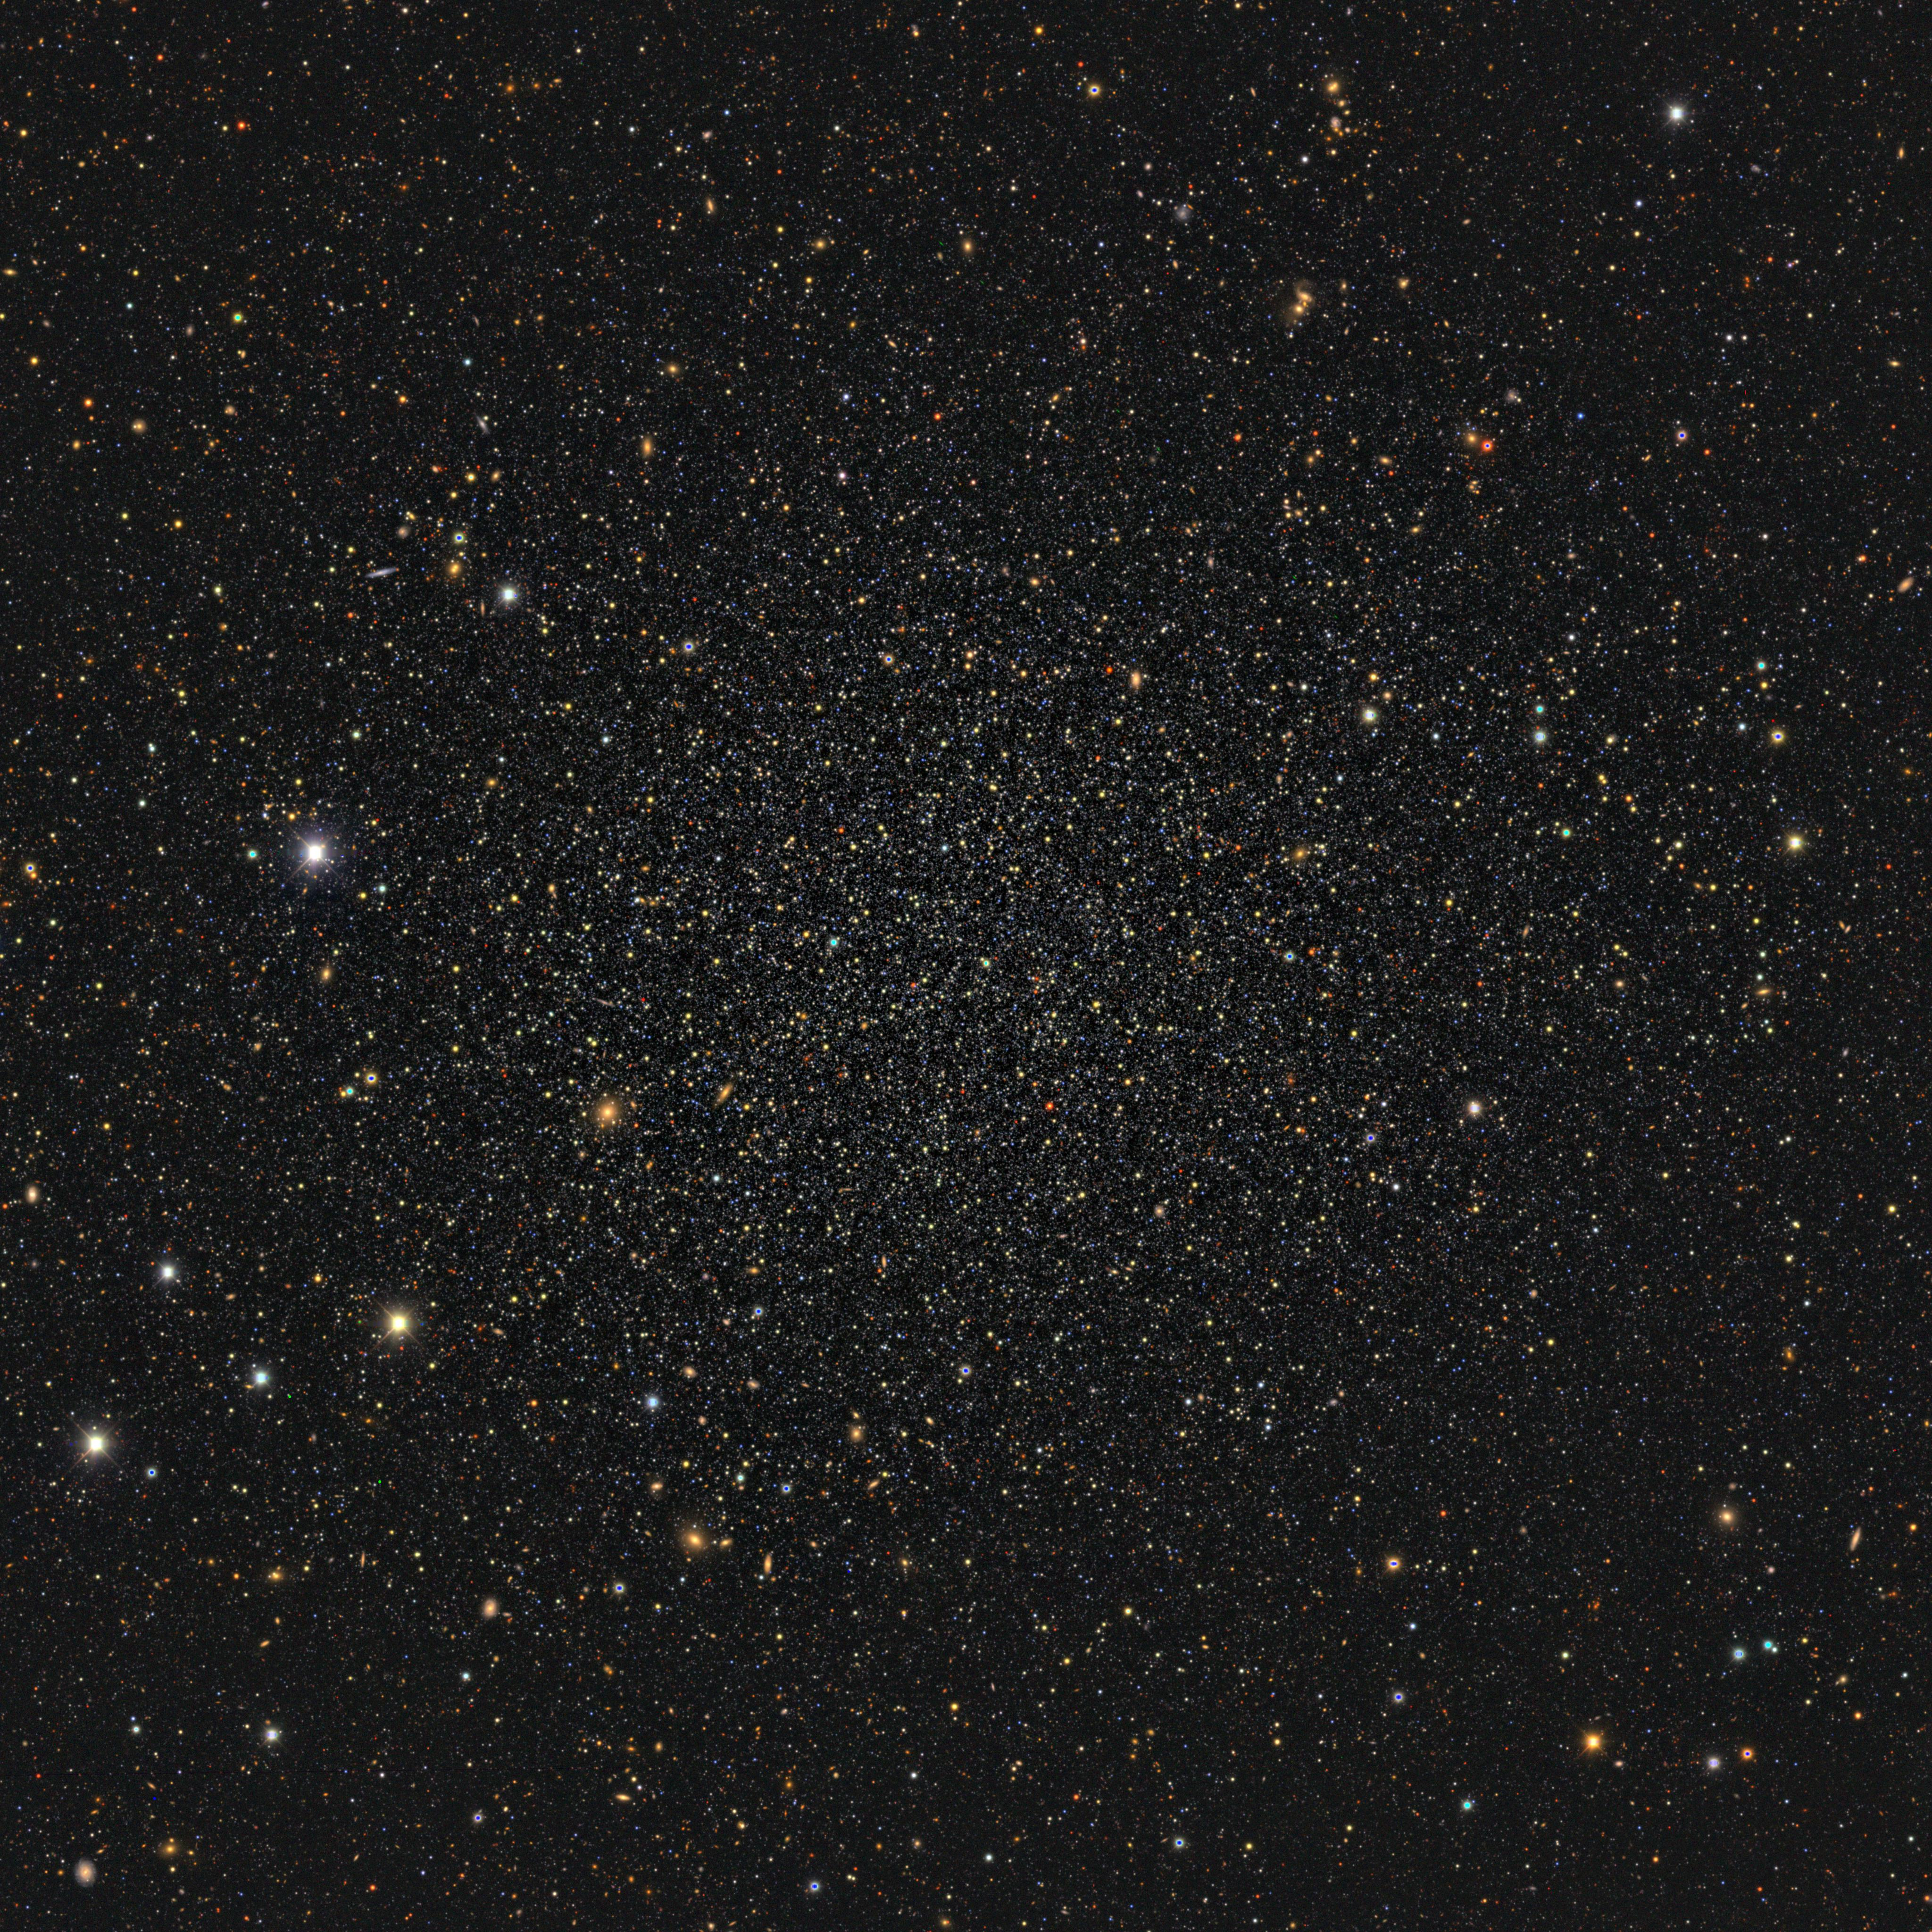
\includegraphics[width=5.41667in,height=5.41667in]{figures/scl_des_dr2.png}
\caption[Picture of Sculptor]{Sculptor image from DES DR 2 via
HiPS2FITS.}\label{fig:scl_image}
\end{figure}

\begin{figure}
\centering
\pandocbounded{\includegraphics[keepaspectratio]{figures/scl_umi_vs_penarrubia.pdf}}
\caption[Idealized simulations match Scl and UMi]{Sculptor and UMi's
profiles are well-matched to \citet{PNM2008}.}\label{fig:toy_profiles}
\end{figure}

Sculptor (Scl) is one of the first discovered dwarf galaxies of the
Milky Way (Shapley 1938; only preceded by the SMC and LMC!). As a
classical dwarf spheroidal, Scl is relatively bright and compact.

Since the initial discovery of Scl, most authors have noted that Scl has
a slight ellipticity (\(0.36\)), often attributed to tidal effects.
However, this does not align with the absolute proper motion or orbital
path of the galaxy.

While Scl has a relatively large pericentre (greater than 50kpc),
\citet{sestito+2023a} detect that the galaxy likely has an excess of
stars in the outskirts (past about 60 arcminutes). This excess is
perhaps one of the clearest indications that Scl may be affected by
tides. Here, our goal is to determine if under a \(\Lambda\) CMD
paradigm with DM-only simulations, tidal effects of the Milky Way (or
LMC) may indeed be consistent with these observations, or if these
observations may reveal instead a extended stellar ``halo'' or second
component of the galaxy---illustrating a complex formation for the
galaxy.

Theoretical work on Sculptor

\begin{itemize}
\tightlist
\item
  \citet{battaglia+2008}
\item
  \citet{iorio+2019}
\item
  \citet{amorisco+zavala+deboer2014}
\item
  \citet{battaglia+2008}
\item
  \citet{breddels+2013}
\item
  \citet{breddels+helmi2013}
\item
  \citet{richardson+fairbairn2014}
\item
  \citet{SFW2017}
\item
  \citet{innanen+papp1979}
\end{itemize}

Observational work on Scl

\begin{itemize}
\tightlist
\item
  \citet{sestito+2023a}
\item
  \citet{tolstoy+2023}, \citet{arroyo-polonio+2023},
  \citet{arroyo-polonio+2024}
\item
  \citet{eskridge1988}, \citet{eskridge1988a}, \citet{eskridge1988b}
\item
  \citet{coleman+dacosta+bland-hawthorn2005}
\item
  \citet{DQ1994}
\item
  \citet{WMO2009}
\item
  \citet{IH1995}, \citet{munoz+2018}
\item
  \citet{kirby+2009}
\item
  \citet{martinez-vazquez+2015}, \citet{pietrzynski+2008}
\end{itemize}

\begin{table*}[t]
\centering
\caption{Measured properties of Sculptor}
\label{tbl:Measured-properties-of-Sculptor}
\begin{tabular}{lll}
\toprule
parameter & value & Source\\
\midrule
$\alpha$ & $15.0183 \pm 0.0012$˚ & M+18\\
$\delta$ & $-33.7186 \pm 0.00072$˚ & M+18\\
distance & $83.2 \pm 2$ kpc & Tran+22\\
$\mu_\alpha \cos \delta$ & $0.099 \pm 0.002 \pm 0.017$ mas yr$^{-1}$ & MV20a\\
$\mu_\delta$ & $-0.160 \pm 0.002_{\rm stat} \pm 0.017_{\rm sys}$ mas yr$^{-1}$ & MV20a\\
RV & $111.2 \pm 0.2$ & arroyo-polonio+24\\
$\sigma_v$ & $9.7\pm0.2$ & arroyo-polonio+24\\
$R_h$ & $12.33 \pm 0.05$ arcmin & MV20*\\
$R_{h,inner}$ & $8.69 \pm 0.2$ arcmin & this work?\\
ell & $0.36 \pm 0.01$ & M+18\\
PA & $92\pm1$ & M+18\\
$M_V$ & $-10.82\pm0.14$ & M+18\\
\bottomrule
\end{tabular}
\end{table*}

Can I just cite \citet{arroyo-polonio+2024} for velocity information for
Sculptor? They correct for binary and do a more detailed discussion of
rotation.

\subsection{Ursa Minor}\label{ursa-minor}

\begin{itemize}
\item
  \citet{sestito+2023b}
\item
  \citet{pace+2020}
\item
  \citet{bellazzini+2002}
\item
  \citet{hargreaves+1994}
\item
  \citet{martinez-delgado+2001}
\item
  \citet{munoz+2005}
\item
  \citet{pace+2020}
\item
  \citet{palma+2003}
\item
  \citet{spencer+2018}
\item
  \citet{vitral+2023}
\end{itemize}

\begin{figure}
\centering
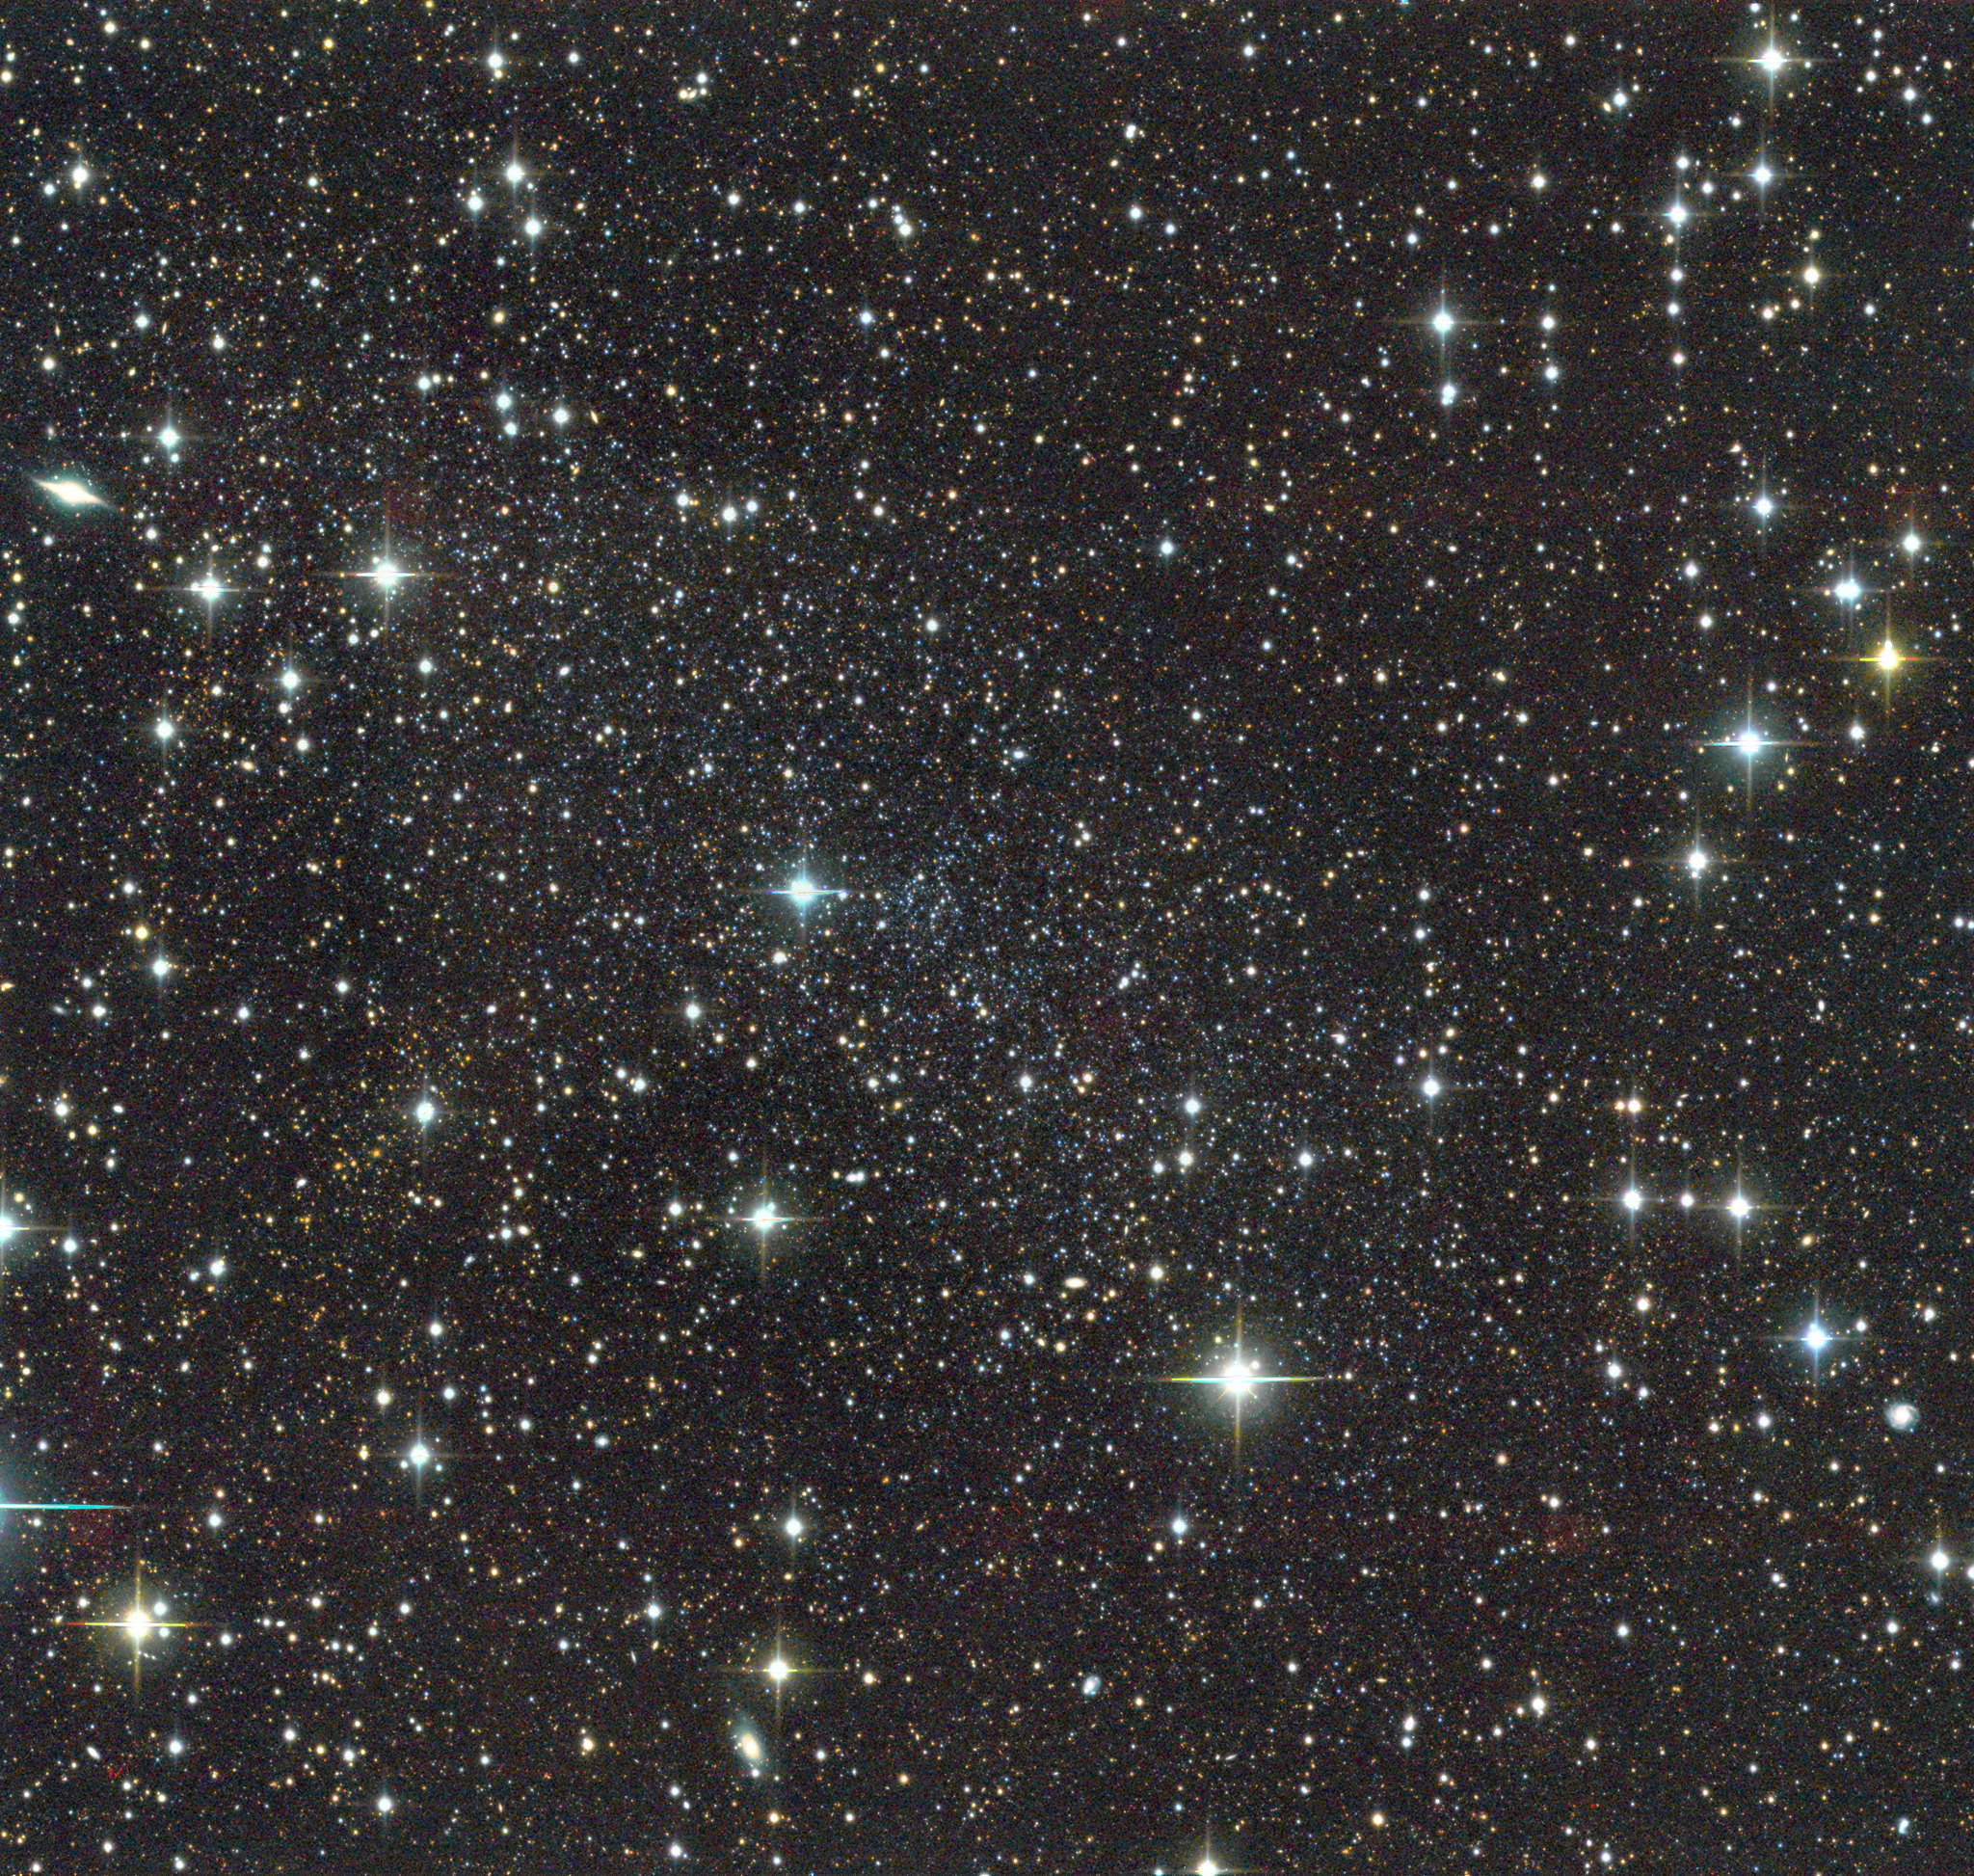
\includegraphics[width=5.41667in,height=5.41667in]{figures/umi_image.jpg}
\caption[Picture of Ursa Minor]{Ursa Minor Dwarf. Composite Public
data/Giuseppe Donatiello. Updated image in 2022.
https://www.flickr.com/photos/133259498@N05/page8}\label{fig:umi_image}
\end{figure}

\begin{table*}[t]
\centering
\caption{Measured properties of Ursa Minor. References are: (1) Muñoz et al. (2018), (2) Garofalo et al. (2025), (3) McConnachie and Venn (2020), (4) average of Pace et al. (2020) and Spencer et al. (2018).}
\label{tbl:Measured-properties-of-Ursa-Minor-References-are:-1-Muñoz-et-al-2018-2-Garofalo-et-al-2025-3-McConnachie-and-Venn-2020-4-average-of-Pace-et-al-2020-and-Spencer-et-al-2018}
\begin{tabular}{lll}
\toprule
parameter & value & Source\\
\midrule
$\alpha$ & $ 227.2420 \pm 0.0045$˚ & 1\\
$\delta$ & $67.2221 \pm 0.00158$˚ & 1\\
distance modulus & $19.23 \pm 0.11$ & 2\\
distance & $70.1 \pm 3.6$ kpc & \\
$\mu_\alpha \cos \delta$ & $-0.124 \pm 0.004 \pm 0.017$ mas yr$^{-1}$ & 3\\
$\mu_\delta$ & $0.078 \pm 0.004_{\rm stat} \pm 0.017_{\rm sys}$ mas yr$^{-1}$ & 3\\
RV & $-244.9 \pm 0.3_{\rm stat} \pm 1.7_{\rm sys}$ km s$^{-1}$ & 4\\
$\sigma_v$ & $8.3 \pm 0.3_{\rm stat} \pm 0.4_{\rm sys}$ & 4\\
$r_h$ & $18.2 \pm 0.1$ arcmin & 1\\
ell & $0.55 \pm 0.01$ & 1\\
PA & $50 \pm 1^\circ$ & 1\\
$M_V$ & $-9.03 \pm 0.05$ & 1\\
\bottomrule
\end{tabular}
\end{table*}

\subsection{Theoretical Background}\label{theoretical-background}

\begin{itemize}
\tightlist
\item
  Cosmology foundations

  \begin{itemize}
  \tightlist
  \item
    power spectrum plot
  \end{itemize}
\item
  NFW plot (density or energy), maybe borrow from paper?

  \begin{itemize}
  \tightlist
  \item
    Explain origin of NFW
  \end{itemize}
\item
  Dwarf galaxy formation, halos
\end{itemize}

N-body DM simulations

\begin{itemize}
\tightlist
\item
  Collisionless Boltzmann equation and meaning of such simulations
\item
  Assumptions \& context \& past work
\item
  Evolution under tidal field
\end{itemize}

To motivate why a tidal interaction may give rise to the observed
density profiles, we create a toy simulation following \citet{PNM2008}.

\begin{itemize}
\item
  NFW initial conditions (sculptor like, vcm, rcm)
\item
  Evolved in x-y plane using \citet{EP2020} potential for
  \textasciitilde{} 5Gyr with pericentre of 15 kpc and apocentre of 100
  kpc.
\item
  Exponential initial stellar profile.
\end{itemize}

As a dark matter halo is perturbed on a pericentric passage with the
milky way,

\begin{itemize}
\tightlist
\item
  Tidal stress heats halo slightly
\item
  Mass loss, particularly of loosely bound particles
\end{itemize}

The stellar component tracers will similarly follow the behaviour of the
dark matter.

An emperical estimate of where the simulation's stars are becoming
unbound is, as stated in \citet{PNM2008}, the break radius \[
R_b = C\,\sigma_{v}\,\Delta t
\] where \(\sigma_v\) is the present line of sight velocity dispersion ,
\(\delta t\) is the time since pericentre, and \(C \approx 0.55\) is a
fit. The idea motivating this equation is stars in the inner regions
will have dynamically equilibriated to the new potential (phase mixed),
however the outer regions are no longer in steady state, so we have to
wait until the crossing time reaches them as well.

As illustrated in fig.~\ref{fig:toy_profiles}, the density profile
initially stars off exponential. At increasing times since the first
pericentric passage, the break radius, appearing as an apparent
separation between the slopes of the inner and outer profile, increases.

\subsection{Introduction to Dark Matter
simulations}\label{introduction-to-dark-matter-simulations}

In this section, we will cover

\begin{itemize}
\tightlist
\item
  How are dark matter simulations conducted
\item
  Interpretations and uncertainties
\item
  Methods
\end{itemize}

\begin{figure}
\centering
\pandocbounded{\includegraphics[keepaspectratio]{/Users/daniel/thesis/figures/idealized_break_radius.png}}
\caption[Break radius validation]{The break radius of the simulations is
set by}\label{fig:idealized_break_radius}
\end{figure}

From this argument, we note that the following properties must be
approximately true for tides to occur:

\begin{itemize}
\tightlist
\item
  Close enough pericentre. The other break radius \(r_J\) implies that
  if the host density is 3x the satellite, stars will be lost
\item
  Corresponding time since last pericentre: If the time since last
  pericentre is not \(\sim\) consistent with an observed break in the
  density profile, then tides
\item
  Halo evolution. As found in \citet{EN2021}, galaxies evolve along well
  defined tidal tracks (assuming spherical, isotropic, NFW halo, which
  may not be true, see \ldots). These tracks tend to ``puff up'' the
  stellar component while also removing dark matter mass, leaving a
  smaller, compacter DM halo with a more extended stellar component.

  \begin{itemize}
  \tightlist
  \item
    This information is mostly related to the statistical initial
    distribution of satellites from cosmology {[}ludlow+2016;
    \citet{fattahi+2018}{]}
  \end{itemize}
\end{itemize}

\subsection{Potentials}\label{potentials}

From the \citet{nfw1996} paper, eqns. 3 \& 4 \[
\frac{\rho}{\rho_c} = \frac{\delta_c}{(r/r_s)(1+r/r_s)^2}
\] where \[
\delta_c = \frac{200}{3}\frac{c^3}{[\ln(1+c)-c/(1+c)]}
\] \(c\) is concentration parameter, \(\rho_c\) is the critical density
of the universe, and \(r_s\) is the characteristic scale length of the
halo.

The NFW halo is sometimes described by \(M_{200}\). \(r_{200}\) is the
radius at which the mean density of the halo interior to \(r_{200}\) is
200 times the critical density of the universe, and \(M_{200}\) is the
mass contained inside \(r_{200}\). As equations: \[
\rho_{200} = 200\rho_{c} = \frac{M_{200}}{(4\pi/3) r_{200}^3}
\]

\[
r_{200} = \sqrt[3]{\frac{1}{200}\frac{3M_{200}}{4\pi \rho_{\rm c
}}}
\]

\[
M_{200} = \frac{4\pi}{3} r_{200}^3\ \rho_{200}
\]

\(M_{200}\) is also sometimes called the virial mass of the halo.
\(r_{200}\) is directly related to \(r_s\) by \[
r_{200} = c\,r_s
\]

Another useful definition is \[
A(x) \equiv \log (1+x) - \frac{x}{1+x}.
\]

We will also define a dimensionless radius \[
x \equiv r/r_s.
\]

A simple substitution to the definition gives

\[
\rho(x) =  \frac{\rho_s/3}{x\ (1+x)^2}
\] where \[
\rho_s = \frac{c^3}{A(c)} \rho_{200}
\] and \(A(c)\) is as above. The characteristic density can also be
written in terms of scale mass, \(M_s = M_{200}/{A(c)}\) (see below),
giving \[
\rho_s = \frac{c^3}{A(c)} \frac{M_{200}}{(4\pi/3)\ r_{200}^3}  = \frac{3M_s}{4\pi\, {r_s}^3}
\] Note that the NFW density profile is the same as an alpha-beta-gamma
profile where \(\alpha=\gamma=1\) and \(\beta =3\).

\subsubsection{Circular velocity}\label{circular-velocity}

The circular velocity in terms of
\(v_{200} = \sqrt{G M_{200} / R_{200}}\) is \[
\left(v_{\rm circ}/v_{200}\right)^2 = \frac{A(x)/x}{A(c)/c},
\]

or in terms of \(M_s\) and \(r_s\), \[
v_{\rm circ}^2 = \frac{G M(r)}{r} = \frac{G M_s A(r/r_s)}{r}.
\] Another parameterization of the NFW profile is in terms of the
maximum circular velocity \(v_{\rm circ}^{\rm max}\) and the radius at
which it is reached \(r_{\rm circ}^{\rm max}\). Given the scale radius,
\[
r_{\rm circ}^{\rm max} = \alpha\ r_s
\]

where \(\alpha\approx2.16258\), and \(v_{\rm circ}^{\rm max}\) can be
found from either of the equations above.
